
\section{FILIP BRODACZ}

Zaistniała zmiana chciałbym punkcika :D
Model bryły sztywnej używany często na fizyce to tylko nierzeczywiste przybliżenie. Ciała rzeczywiste ulegają bowiem zniekształceniu pod wpływem przyłożonych sił.

	
Co oznacza, że sila jest proporcjonalna do wydłużenia. Definiujemy:
	\textbf{Moduł sprężystości} – stosunek naprezenia  do odkształcenia względnego\\
	\textbf{Naprężenie} - stosunek przyłożonej siły do pola powierzchni przekroju ciała\\


Rozwazmy rozciaganie jednorodnego preta:
\begin{figure}[htbp]
    \centering
    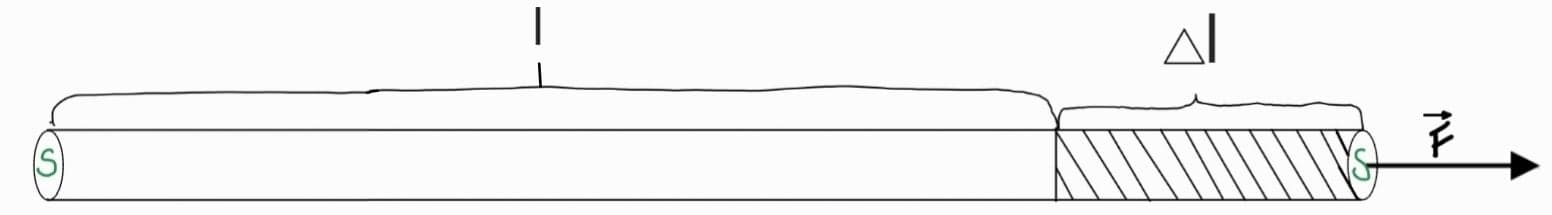
\includegraphics[width=0.2\textwidth]{pictures/pret.jpg}
    \caption{Pomocniczy rysunek prezentujacy rozciagajacy sie pret}
    \label{rys1}
\end{figure}

\begin{quote}
    \empth{Odkształcenie względne jest proporcjonalne do ciśnienia.} [4] 
\end{quote}
Więc rozciągnięcie drutu wyraża się wzorem: 
\begin{equation}\label{eq1}
 \Delta l = k \cdot \frac{F \cdot l}{S}
\end{equation}

Wychodzimy ze wzoru (1) i chcemy otrzymać wzór na ogólne \underline{prawo Hooke’a}.
\begin{center}
$ \Delta l $ – wydłużenie bezwzględne \\
$F$ – siła \\
$l$ – długość początkowa\\
$S$– pole przekroju poprzecznego\\
\end{center}

\newpage
Do pomiarów:

\begin{itemize}
    \item Śruba mikrometryczna, o podziałce 0.01 mm, zakres $\left[0;15mm\right]$
    \item Metrówka o podziałce 1cm, zakres $\left[0;150cm\right]$
\end{itemize}

Oraz

\begin{enumerate}
    \item Waga o podziałce 1g, zakres $\left[0;4kg\right]$
    \item Mikrometr o podziałce $0.01mm$, zakres $\left[0;1cm\right]$
\end{enumerate}

\begin{table}[!h]
\centering
\begin{tabular}{|p{2cm}|p{2cm}|p{2cm}|p{2cm}|p{2cm}|p{2cm}|p{2cm}|} \hline
Pomiar & Masa odważników [kg] & Siła F [N] & Wskazanie czujnika $\uparrow$ [mm] & Wskazanie czujnika $\downarrow$ [mm] & Wydłużenie średnia $\Delta l $[mm] \\ \hline
 $1$   & $0.499$  & $4.90$ & $0.13$ & $0.15$ & $0.14$  \\ \hline
 $2$   & $0.998$  & $9.79$ & $0.27$ & $0.29$ & $0.28$  \\ \hline
 $3$   & $1.498$  & $14.7$ & $0.4$  & $0.42$ & $0.41$  \\ \hline
 $4$   & $1,997$  & $19.6$ & $0.56$ & $0.57$ & $0.565$ \\ \hline
 $5$   & $2,497$  & $24.5$ & $0.7$  & $0.71$ & $0.705$ \\ \hline
 $6$   & $2,996$  & $29.4$ & $0.84$ & $0.84$ & $0.84$  \\ \hline
\end{tabular}
\caption{Dane pomiarowe-Stal\label{tab1}}
\end{table}

Jak widzimy tabela \ref{tab1} informuje nas jak bardzo rozciągnął sie drut stalowy pod wpływem siły, która na rysunku \ref{rys1} jest oznaczona literą $F$
